%! TEX root = ../main.tex
\documentclass[main]{subfiles}

\begin{document}
\chapter{本論}
私が星空写真を始めたときに躓いたところを細かく説明しながら簡単に星が撮れることを説明しようと記事を書いていたらとても長く,まとまりがつかなくなったので,いくつか割愛・抜粋して付録としてお届けします.別の機会にすべてお伝えできたらいいなと考えています.
\section{星空写真の種類}
星空をメインにした写真には大きく分けて次の3種類が挙げられます.
\subsection{星景写真}
\begin{itemize}
    \item 広角で星空と風景の両方の写真が写っている写真のこと
    \item 比較的撮影の難易度が低い
    \item カメラと三脚があれば今すぐにでも試せる
\end{itemize}
\subsection{星野写真}
\begin{itemize}
    \item 標準~中望遠程度の画角で星空のみ,星座などが中心の写真
    \item ISO感度を上げればカメラと三脚だけでも撮れないことはない.
    \item 本格的に撮るとなれば,ポータブル赤道儀など専門的な機材が必要
\end{itemize}
\subsection{天体写真}
\begin{itemize}
    \item 望遠~超望遠で惑星や星雲・銀河などが主役になる写真
    \item 赤道儀と天体望遠鏡が必須
    \item 撮影方法やその後の処理含めて必要な機材が多くて複雑
\end{itemize}
\section{初心者はまず星景写真から}
星空観測を楽しむためには,天体望遠鏡が必要だと考える人も多いでしょう.天体望遠鏡を使えば月や惑星,星雲や銀河などを観察したり撮影できます.しかし,そういった天体望遠鏡は非常に高価だったり,よく選ばずに安価なものを買うと何も見えず満足に楽しめないこともあり初心者には特にハードルが高く感じるでしょう.そのため,まずは手軽に星空観測を楽しむ方法として,カメラと三脚さえあれば始められる星景写真を紹介します.

星景写真は,広角レンズを使用して,星空と風景を一緒に写した写真です.星空観測と同様に,撮影する場所や時間帯が重要です.また,カメラの設定が重要で,マニュアルモードでの撮影がおすすめです.露出時間やISO感度,絞りなどを調整することで,美しい星空写真を撮影できます.

\begin{tcolorbox}[title=星景写真に必要な物, breakable]
    \begin{description}
        \item[カメラ:]この後にも詳しく説明しますが,マニュアル設定ができるカメラが必要です.
        \item[三脚:]長時間露光をするために,カメラを固定する三脚が必要です.なるべく脚が太くて耐荷重の大きい物が良いです.特にカーボン製でセンターポールのないものがおすすめ.
        \item[リモートシャッター:]リモートシャッターを使用することで,カメラを手で触ることなくシャッターを切ることができます.三脚を使っていても,長時間露光をする星景写真では,シャッターボタンを直接押して撮影するのは被写体ブレにつながってしまいます.リモコンやスマホなどでシャッターを切るか,タイマー機能を利用しましょう.
        \item[星空観望の必需品] \mbox{}\\
            \begin{description}
                \item[防寒具:] 外で長時間過ごすため,防寒具が必要です.星景写真を撮影する場合,晴れた夜空の下では放射冷却によって地面から冷気が上がってくるように寒くなります.家を出るときは着すぎず,汗ばむ程度がちょうどいいです.ただし,汗ばんだままだと体温を下げてしまうので,服選びでは保温性に加えて透湿性にも注意しましょう.足元が冷たくなるため,スノーブーツと雪用靴下を履くことをおすすめします.\mbox{}\par
                    例えば,肌着にエアリズムを着用し,厚手のヒートテック,フリース,そしてダウンを重ね着することで,防寒性を高めながら透湿性も確保できます.ただし,着込みすぎても熱が奪われてしまうため,適度な空気の層を取り込んでおくことが大切です.着込みすぎると動きにくく,むしろ熱が奪われやすくなります.
                \item[ヘッドランプ:] 夜間に撮影する場合,手元が暗くなるため,ヘッドランプが必要です.ヘッドランプを使用することで,手元を照らし,操作をスムーズに行うことができます.(赤色か電球色の弱めのライトがおすすめ:暗順応)
                \item[行動食:] 星空観望の一番の敵は真夜中の寒さです.防寒着ももちろん大切ですが,体の内側から熱を生み出すために軽食や水分の補給も必要です.チョコを含んだお菓子や温かい紅茶などを準備していくといいでしょう.
                \item[スマートフォン:] 星座表や懐中電灯代わりにもなりますし,非常時の連絡や地図の確認などで必要不可欠です.また,星空撮影では撮影の間かなり暇を持て余すので暇つぶしにも必要です.
            \end{description}
    \end{description}
\end{tcolorbox}

\begin{figure}[htbp]
    \centering
    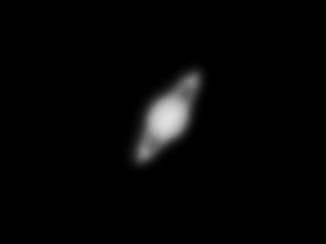
\includegraphics[keepaspectratio, width=\linewidth]{figures/Saturn.jpg}
    \caption{caption}
    \label{fig:label}
\end{figure}

\end{document}